\section{Guía de estilos y sistema de diseño}
\label{sec:guia_estilos}

Para garantizar una experiencia de usuario consistente, intuitiva y accesible en todas las vistas de la plataforma, se ha formalizado una guía de estilos fundamentada en un sistema de diseño (\emph{Design System}) centralizado. Este sistema estandariza los componentes visuales a partir de la metodología \emph{Atomic Design} de Brad Frost, descomponiendo la interfaz desde los elementos más básicos (\emph{design tokens} de color y tipografía) hasta moléculas interactivas reutilizables (botones, barras de búsqueda, selectores y contenedores).

La figura \ref{fig:guia_estilos} sintetiza las directrices visuales maestras implementadas para la plataforma Colivi en Figma, asegurando armonía estética y reduciendo la carga cognitiva del usuario.

\begin{figure}[H]
    \centering
    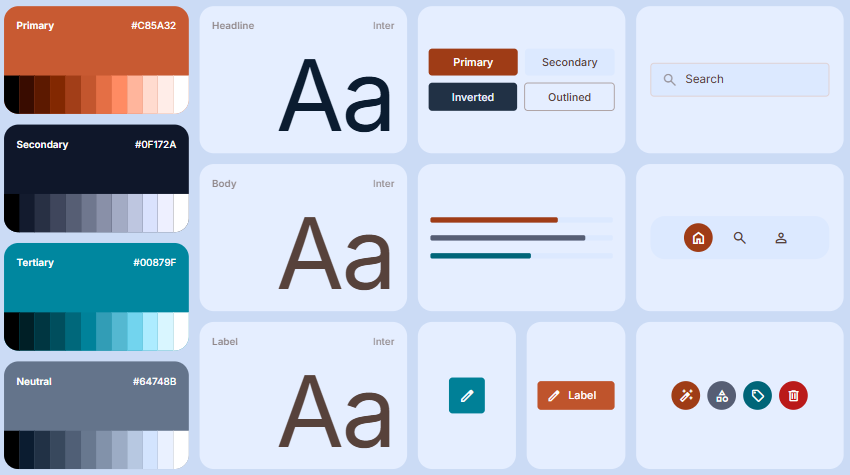
\includegraphics[width=0.92\textwidth]{AnalisisFuncional/img/guia_estilos.png}
    \caption{Guía de estilos, tokens de diseño y componentes atómicos de Colivi. Elaboración propia}
    \label{fig:guia_estilos}
\end{figure}

\subsection{Paleta cromática y tokens de color}

El esquema de color combina tonos terrosos y marinos que transmiten cercanía, habitabilidad y profesionalidad, cumpliendo con los estándares de contraste exigidos por las pautas de accesibilidad WCAG 2.1. Cada color principal cuenta con una rampa tonal escalonada para resolver estados de interacción (\emph{hover}, \emph{active}, \emph{disabled}):

\begin{table}[H]
    \centering
    \begin{tabular}{|p{2cm}|p{1.8cm}|p{4.2cm}|p{5cm}|}
        \hline
        \textbf{Token} & \textbf{Hex} & \textbf{Rol en el sistema} & \textbf{Elementos asignados} \\ \hline
        \textbf{Primary} & \texttt{\#C85A32} & Marca principal (Terracota cálido) & Botones principales (CTA), pestañas activas, chips destacados e indicadores. \\ \hline
        \textbf{Secondary} & \texttt{\#0F172A} & Contraste estructural (Slate 900) & Titulares principales (\emph{Headlines}), texto de máximo contraste y botones invertidos. \\ \hline
        \textbf{Tertiary} & \texttt{\#00879F} & Tono funcional (Azul petróleo / Teal) & Iconos de edición, acentos complementarios, filtros activos y progreso secundario. \\ \hline
        \textbf{Neutral} & \texttt{\#64748B} & Soporte neutro (Slate 500) & Bordes de tarjetas, líneas divisorias, texto secundario y fondos inactivos. \\ \hline
        \textbf{Destructive} & \texttt{\#B91C1C} & Alerta y criticidad (Rojo intenso) & Acciones de borrado (icono papelera), bajas y mensajes de error. \\ \hline
    \end{tabular}
    \caption{Definición de tokens cromáticos y asignación semántica en Colivi}
    \label{tab:tokens_cromaticos}
\end{table}

\subsection{Jerarquía tipográfica}

Para la tipografía corporativa se ha seleccionado la fuente de palo seco (\emph{sans-serif}) \textbf{Inter}, concebida específicamente para interfaces de usuario en pantallas digitales. Su elevada altura de la x (\emph{x-height}) y la diferenciación nítida de sus glifos garantizan una legibilidad óptima tanto en monitores de escritorio como en terminales móviles de reducidas dimensiones.

El sistema establece tres niveles tipográficos esenciales:
\begin{itemize}
    \item \textbf{Headline (Titulares):} Fuente Inter en peso \emph{Bold} / \emph{SemiBold} y color secundario (\texttt{\#0F172A}). Aporta jerarquía visual a encabezados de sección y títulos de inmuebles.
    \item \textbf{Body (Cuerpo de texto):} Fuente Inter en peso \emph{Regular} con interlineado a 1.5 y contraste atenuado, optimizado para lectura continuada sin fatiga visual.
    \item \textbf{Label (Etiquetas y controles):} Fuente Inter en peso \emph{Medium}. Formato compacto para textos de botones, campos de entrada, selectores y microetiquetas informativas.
\end{itemize}

\subsection{Componentes atómicos e interactivos}

A partir de los tokens de color y tipografía se articula la biblioteca de componentes atómicos:

\begin{itemize}
    \item \textbf{Botones y llamadas a la acción:}
    \begin{itemize}
        \item \emph{Primary:} Fondo terracota (\texttt{\#C85A32}) y texto blanco con bordes redondeados (radio de 8px). Se reserva exclusivamente para la acción dominante de la pantalla (p. ej., «Reservar alojamiento», «Crear hogar»).
        \item \emph{Secondary:} Fondo azul claro desaturado y texto oscuro para acciones accesorias o de navegación intermedia.
        \item \emph{Inverted:} Fondo marino profundo (\texttt{\#0F172A}) para destacar sobre contenedores de contraste o cabeceras.
        \item \emph{Outlined:} Fondo transparente y contorno neutro (\texttt{\#64748B}) para acciones de cancelación o retroceso.
    \end{itemize}

    \item \textbf{Campos de búsqueda e introducción de datos:} Contenedores rectangulares redondeados con icono semántico de lupa (\emph{Search}), bordes suaves y fondo neutro para evitar sobrecarga visual al rellenar formularios.

    \item \textbf{Barras de progreso y acentos visuales:} Líneas horizontales coloreadas en la tríada cromática (Terracota, Marino y Teal) para comunicar métricas relativas (grado de completitud de perfil, porcentaje de gasto cubierto o progreso de tareas).

    \item \textbf{Navegación tipo cápsula (\emph{Pills Navigation}):} Barra compacta con iconos vectoriales (Inicio, Explorador y Perfil), destacando la vista activa mediante un círculo contenedor en color primario.

    \item \textbf{Insignias y botones flotantes de acción rápida:} Chips de etiquetado con icono y texto explicativo, y botones circulares de acción directa identificados por su iconografía (herramientas mágicas del asistente IA, categorías, etiquetas de filtro y eliminación destructiva).
\end{itemize}

\subsection{Ergonomía espacial y accesibilidad}

El sistema adopta una retícula base de 8 puntos (\emph{8-point grid}), donde todos los márgenes, rellenos (\emph{padding}) y dimensiones de componentes son múltiplos exactos de 8px (o múltiplos de 4px para microespaciados en iconos y badges). Esta disciplina matemática asegura que los elementos se redimensionen de manera armónica en cualquier resolución de pantalla (\hyperref[tab:requisitos-no-funcionales]{RNF-06}).

Asimismo, los contrastes entre texto y fondo superan el ratio mínimo de 4.5:1 exigido para el nivel AA de la norma WCAG 2.1, garantizando la accesibilidad para usuarios con diversidad visual o condiciones de iluminación desfavorables.

